\documentclass[11pt]{article}
\usepackage[margin=0.9in]{geometry}
\usepackage{tikz}
\usepackage{xcolor}
\usepackage[hidelinks]{hyperref}
\usepackage{enumitem}
\definecolor{ink}{HTML}{1F2933}
\definecolor{soft}{HTML}{D9DEE3}
\definecolor{teal}{HTML}{0F766E}
\definecolor{rose}{HTML}{BE123C}
\color{ink}
\setlength{\parindent}{0pt}
\setlength{\parskip}{7pt}
\tikzset{normal/.style={fill=soft}, double/.style={fill=teal}, empty/.style={fill=white, draw=rose, line width=0.7pt}}
\newcommand{\key}[1]{\tikz[baseline=-0.6ex]\fill[#1] (0,-0.12) rectangle (0.24,0.12);}

\begin{document}
\pagestyle{empty}

{\LARGE\bfseries Quiet Collisions}\\[3pt]
{\large A small math result, explained without math}\\[2pt]
{\small Ayomide (Daniel) Shittu \;·\; November 2026}

\vspace{6pt}
\section*{The story: a mail sorter}

Picture a building with \textbf{1{,}024 people} and \textbf{1{,}024 mailboxes}.
A sorting machine is supposed to give every person their own box. If the
machine is faulty, some boxes get two people's mail and other boxes get none.
I call each of these mix-ups a \emph{collision}.

Every mailbox address is made of \textbf{10 yes/no labels}: east or west wing,
upper or lower floor, front or back, and so on. Nobody can check all 1{,}024
boxes, so inspectors take shortcuts. Each inspector picks \textbf{a few labels}
and checks that the mail is spread evenly across them. For example, ``Do the
east and west wings get the same amount of mail?''

\textbf{The question:} can a broken machine pass every small inspection? If it
can, how broken does it have to be?

\section*{The answer}

I found the exact answer, and it is the larger of two numbers:

\begin{center}
\fbox{\parbox{0.86\linewidth}{\centering\vspace{3pt}
\textbf{Least possible damage} \;=\; the bigger of\\[3pt]
\textbf{(1)} what it takes to fool inspectors who look at that many labels, and\\
\textbf{(2)} what it takes to be broken at all, for a machine built from simple parts.
\vspace{3pt}}}
\end{center}

\begin{itemize}[leftmargin=1.4em, itemsep=3pt]
\item \textbf{Reason 1: hiding spreads the damage out.} To look balanced to
every small inspection, the mistakes must be spread over many boxes. One or
two wrong boxes would get caught.
\item \textbf{Reason 2: simple machines can't make small mistakes.} A machine
built from the simplest kind of parts is either perfect or noticeably off.
There is no ``slightly broken.''
\end{itemize}

Here \emph{damage} means the number of wrong mailboxes, with a box that is
off by more than one letter counting extra.

The two reasons never interfere with each other. Whichever is stronger sets
the answer. I also \textbf{built a machine that hits that minimum exactly}, so the
answer can't be improved.

\newpage
\section*{What it looks like}

Here is that machine for the 1{,}024-box building, with inspectors who may look
at up to 4 labels at once. Each square is one mailbox.

\begin{center}
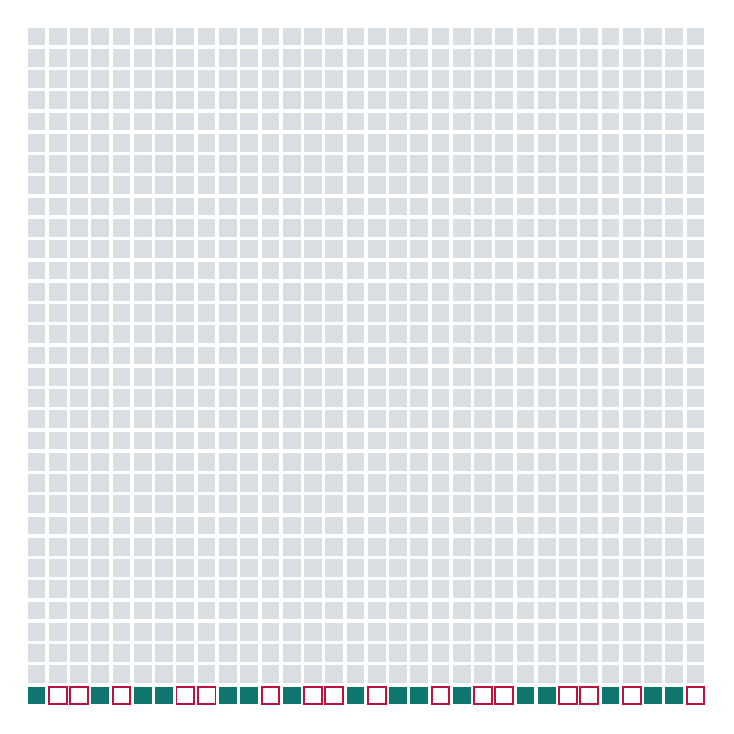
\begin{tikzpicture}
\fill[normal] (0.000,8.370) rectangle ++(0.225,0.225);
\fill[normal] (0.270,8.370) rectangle ++(0.225,0.225);
\fill[normal] (0.540,8.370) rectangle ++(0.225,0.225);
\fill[normal] (0.810,8.370) rectangle ++(0.225,0.225);
\fill[normal] (1.080,8.370) rectangle ++(0.225,0.225);
\fill[normal] (1.350,8.370) rectangle ++(0.225,0.225);
\fill[normal] (1.620,8.370) rectangle ++(0.225,0.225);
\fill[normal] (1.890,8.370) rectangle ++(0.225,0.225);
\fill[normal] (2.160,8.370) rectangle ++(0.225,0.225);
\fill[normal] (2.430,8.370) rectangle ++(0.225,0.225);
\fill[normal] (2.700,8.370) rectangle ++(0.225,0.225);
\fill[normal] (2.970,8.370) rectangle ++(0.225,0.225);
\fill[normal] (3.240,8.370) rectangle ++(0.225,0.225);
\fill[normal] (3.510,8.370) rectangle ++(0.225,0.225);
\fill[normal] (3.780,8.370) rectangle ++(0.225,0.225);
\fill[normal] (4.050,8.370) rectangle ++(0.225,0.225);
\fill[normal] (4.320,8.370) rectangle ++(0.225,0.225);
\fill[normal] (4.590,8.370) rectangle ++(0.225,0.225);
\fill[normal] (4.860,8.370) rectangle ++(0.225,0.225);
\fill[normal] (5.130,8.370) rectangle ++(0.225,0.225);
\fill[normal] (5.400,8.370) rectangle ++(0.225,0.225);
\fill[normal] (5.670,8.370) rectangle ++(0.225,0.225);
\fill[normal] (5.940,8.370) rectangle ++(0.225,0.225);
\fill[normal] (6.210,8.370) rectangle ++(0.225,0.225);
\fill[normal] (6.480,8.370) rectangle ++(0.225,0.225);
\fill[normal] (6.750,8.370) rectangle ++(0.225,0.225);
\fill[normal] (7.020,8.370) rectangle ++(0.225,0.225);
\fill[normal] (7.290,8.370) rectangle ++(0.225,0.225);
\fill[normal] (7.560,8.370) rectangle ++(0.225,0.225);
\fill[normal] (7.830,8.370) rectangle ++(0.225,0.225);
\fill[normal] (8.100,8.370) rectangle ++(0.225,0.225);
\fill[normal] (8.370,8.370) rectangle ++(0.225,0.225);
\fill[normal] (0.000,8.100) rectangle ++(0.225,0.225);
\fill[normal] (0.270,8.100) rectangle ++(0.225,0.225);
\fill[normal] (0.540,8.100) rectangle ++(0.225,0.225);
\fill[normal] (0.810,8.100) rectangle ++(0.225,0.225);
\fill[normal] (1.080,8.100) rectangle ++(0.225,0.225);
\fill[normal] (1.350,8.100) rectangle ++(0.225,0.225);
\fill[normal] (1.620,8.100) rectangle ++(0.225,0.225);
\fill[normal] (1.890,8.100) rectangle ++(0.225,0.225);
\fill[normal] (2.160,8.100) rectangle ++(0.225,0.225);
\fill[normal] (2.430,8.100) rectangle ++(0.225,0.225);
\fill[normal] (2.700,8.100) rectangle ++(0.225,0.225);
\fill[normal] (2.970,8.100) rectangle ++(0.225,0.225);
\fill[normal] (3.240,8.100) rectangle ++(0.225,0.225);
\fill[normal] (3.510,8.100) rectangle ++(0.225,0.225);
\fill[normal] (3.780,8.100) rectangle ++(0.225,0.225);
\fill[normal] (4.050,8.100) rectangle ++(0.225,0.225);
\fill[normal] (4.320,8.100) rectangle ++(0.225,0.225);
\fill[normal] (4.590,8.100) rectangle ++(0.225,0.225);
\fill[normal] (4.860,8.100) rectangle ++(0.225,0.225);
\fill[normal] (5.130,8.100) rectangle ++(0.225,0.225);
\fill[normal] (5.400,8.100) rectangle ++(0.225,0.225);
\fill[normal] (5.670,8.100) rectangle ++(0.225,0.225);
\fill[normal] (5.940,8.100) rectangle ++(0.225,0.225);
\fill[normal] (6.210,8.100) rectangle ++(0.225,0.225);
\fill[normal] (6.480,8.100) rectangle ++(0.225,0.225);
\fill[normal] (6.750,8.100) rectangle ++(0.225,0.225);
\fill[normal] (7.020,8.100) rectangle ++(0.225,0.225);
\fill[normal] (7.290,8.100) rectangle ++(0.225,0.225);
\fill[normal] (7.560,8.100) rectangle ++(0.225,0.225);
\fill[normal] (7.830,8.100) rectangle ++(0.225,0.225);
\fill[normal] (8.100,8.100) rectangle ++(0.225,0.225);
\fill[normal] (8.370,8.100) rectangle ++(0.225,0.225);
\fill[normal] (0.000,7.830) rectangle ++(0.225,0.225);
\fill[normal] (0.270,7.830) rectangle ++(0.225,0.225);
\fill[normal] (0.540,7.830) rectangle ++(0.225,0.225);
\fill[normal] (0.810,7.830) rectangle ++(0.225,0.225);
\fill[normal] (1.080,7.830) rectangle ++(0.225,0.225);
\fill[normal] (1.350,7.830) rectangle ++(0.225,0.225);
\fill[normal] (1.620,7.830) rectangle ++(0.225,0.225);
\fill[normal] (1.890,7.830) rectangle ++(0.225,0.225);
\fill[normal] (2.160,7.830) rectangle ++(0.225,0.225);
\fill[normal] (2.430,7.830) rectangle ++(0.225,0.225);
\fill[normal] (2.700,7.830) rectangle ++(0.225,0.225);
\fill[normal] (2.970,7.830) rectangle ++(0.225,0.225);
\fill[normal] (3.240,7.830) rectangle ++(0.225,0.225);
\fill[normal] (3.510,7.830) rectangle ++(0.225,0.225);
\fill[normal] (3.780,7.830) rectangle ++(0.225,0.225);
\fill[normal] (4.050,7.830) rectangle ++(0.225,0.225);
\fill[normal] (4.320,7.830) rectangle ++(0.225,0.225);
\fill[normal] (4.590,7.830) rectangle ++(0.225,0.225);
\fill[normal] (4.860,7.830) rectangle ++(0.225,0.225);
\fill[normal] (5.130,7.830) rectangle ++(0.225,0.225);
\fill[normal] (5.400,7.830) rectangle ++(0.225,0.225);
\fill[normal] (5.670,7.830) rectangle ++(0.225,0.225);
\fill[normal] (5.940,7.830) rectangle ++(0.225,0.225);
\fill[normal] (6.210,7.830) rectangle ++(0.225,0.225);
\fill[normal] (6.480,7.830) rectangle ++(0.225,0.225);
\fill[normal] (6.750,7.830) rectangle ++(0.225,0.225);
\fill[normal] (7.020,7.830) rectangle ++(0.225,0.225);
\fill[normal] (7.290,7.830) rectangle ++(0.225,0.225);
\fill[normal] (7.560,7.830) rectangle ++(0.225,0.225);
\fill[normal] (7.830,7.830) rectangle ++(0.225,0.225);
\fill[normal] (8.100,7.830) rectangle ++(0.225,0.225);
\fill[normal] (8.370,7.830) rectangle ++(0.225,0.225);
\fill[normal] (0.000,7.560) rectangle ++(0.225,0.225);
\fill[normal] (0.270,7.560) rectangle ++(0.225,0.225);
\fill[normal] (0.540,7.560) rectangle ++(0.225,0.225);
\fill[normal] (0.810,7.560) rectangle ++(0.225,0.225);
\fill[normal] (1.080,7.560) rectangle ++(0.225,0.225);
\fill[normal] (1.350,7.560) rectangle ++(0.225,0.225);
\fill[normal] (1.620,7.560) rectangle ++(0.225,0.225);
\fill[normal] (1.890,7.560) rectangle ++(0.225,0.225);
\fill[normal] (2.160,7.560) rectangle ++(0.225,0.225);
\fill[normal] (2.430,7.560) rectangle ++(0.225,0.225);
\fill[normal] (2.700,7.560) rectangle ++(0.225,0.225);
\fill[normal] (2.970,7.560) rectangle ++(0.225,0.225);
\fill[normal] (3.240,7.560) rectangle ++(0.225,0.225);
\fill[normal] (3.510,7.560) rectangle ++(0.225,0.225);
\fill[normal] (3.780,7.560) rectangle ++(0.225,0.225);
\fill[normal] (4.050,7.560) rectangle ++(0.225,0.225);
\fill[normal] (4.320,7.560) rectangle ++(0.225,0.225);
\fill[normal] (4.590,7.560) rectangle ++(0.225,0.225);
\fill[normal] (4.860,7.560) rectangle ++(0.225,0.225);
\fill[normal] (5.130,7.560) rectangle ++(0.225,0.225);
\fill[normal] (5.400,7.560) rectangle ++(0.225,0.225);
\fill[normal] (5.670,7.560) rectangle ++(0.225,0.225);
\fill[normal] (5.940,7.560) rectangle ++(0.225,0.225);
\fill[normal] (6.210,7.560) rectangle ++(0.225,0.225);
\fill[normal] (6.480,7.560) rectangle ++(0.225,0.225);
\fill[normal] (6.750,7.560) rectangle ++(0.225,0.225);
\fill[normal] (7.020,7.560) rectangle ++(0.225,0.225);
\fill[normal] (7.290,7.560) rectangle ++(0.225,0.225);
\fill[normal] (7.560,7.560) rectangle ++(0.225,0.225);
\fill[normal] (7.830,7.560) rectangle ++(0.225,0.225);
\fill[normal] (8.100,7.560) rectangle ++(0.225,0.225);
\fill[normal] (8.370,7.560) rectangle ++(0.225,0.225);
\fill[normal] (0.000,7.290) rectangle ++(0.225,0.225);
\fill[normal] (0.270,7.290) rectangle ++(0.225,0.225);
\fill[normal] (0.540,7.290) rectangle ++(0.225,0.225);
\fill[normal] (0.810,7.290) rectangle ++(0.225,0.225);
\fill[normal] (1.080,7.290) rectangle ++(0.225,0.225);
\fill[normal] (1.350,7.290) rectangle ++(0.225,0.225);
\fill[normal] (1.620,7.290) rectangle ++(0.225,0.225);
\fill[normal] (1.890,7.290) rectangle ++(0.225,0.225);
\fill[normal] (2.160,7.290) rectangle ++(0.225,0.225);
\fill[normal] (2.430,7.290) rectangle ++(0.225,0.225);
\fill[normal] (2.700,7.290) rectangle ++(0.225,0.225);
\fill[normal] (2.970,7.290) rectangle ++(0.225,0.225);
\fill[normal] (3.240,7.290) rectangle ++(0.225,0.225);
\fill[normal] (3.510,7.290) rectangle ++(0.225,0.225);
\fill[normal] (3.780,7.290) rectangle ++(0.225,0.225);
\fill[normal] (4.050,7.290) rectangle ++(0.225,0.225);
\fill[normal] (4.320,7.290) rectangle ++(0.225,0.225);
\fill[normal] (4.590,7.290) rectangle ++(0.225,0.225);
\fill[normal] (4.860,7.290) rectangle ++(0.225,0.225);
\fill[normal] (5.130,7.290) rectangle ++(0.225,0.225);
\fill[normal] (5.400,7.290) rectangle ++(0.225,0.225);
\fill[normal] (5.670,7.290) rectangle ++(0.225,0.225);
\fill[normal] (5.940,7.290) rectangle ++(0.225,0.225);
\fill[normal] (6.210,7.290) rectangle ++(0.225,0.225);
\fill[normal] (6.480,7.290) rectangle ++(0.225,0.225);
\fill[normal] (6.750,7.290) rectangle ++(0.225,0.225);
\fill[normal] (7.020,7.290) rectangle ++(0.225,0.225);
\fill[normal] (7.290,7.290) rectangle ++(0.225,0.225);
\fill[normal] (7.560,7.290) rectangle ++(0.225,0.225);
\fill[normal] (7.830,7.290) rectangle ++(0.225,0.225);
\fill[normal] (8.100,7.290) rectangle ++(0.225,0.225);
\fill[normal] (8.370,7.290) rectangle ++(0.225,0.225);
\fill[normal] (0.000,7.020) rectangle ++(0.225,0.225);
\fill[normal] (0.270,7.020) rectangle ++(0.225,0.225);
\fill[normal] (0.540,7.020) rectangle ++(0.225,0.225);
\fill[normal] (0.810,7.020) rectangle ++(0.225,0.225);
\fill[normal] (1.080,7.020) rectangle ++(0.225,0.225);
\fill[normal] (1.350,7.020) rectangle ++(0.225,0.225);
\fill[normal] (1.620,7.020) rectangle ++(0.225,0.225);
\fill[normal] (1.890,7.020) rectangle ++(0.225,0.225);
\fill[normal] (2.160,7.020) rectangle ++(0.225,0.225);
\fill[normal] (2.430,7.020) rectangle ++(0.225,0.225);
\fill[normal] (2.700,7.020) rectangle ++(0.225,0.225);
\fill[normal] (2.970,7.020) rectangle ++(0.225,0.225);
\fill[normal] (3.240,7.020) rectangle ++(0.225,0.225);
\fill[normal] (3.510,7.020) rectangle ++(0.225,0.225);
\fill[normal] (3.780,7.020) rectangle ++(0.225,0.225);
\fill[normal] (4.050,7.020) rectangle ++(0.225,0.225);
\fill[normal] (4.320,7.020) rectangle ++(0.225,0.225);
\fill[normal] (4.590,7.020) rectangle ++(0.225,0.225);
\fill[normal] (4.860,7.020) rectangle ++(0.225,0.225);
\fill[normal] (5.130,7.020) rectangle ++(0.225,0.225);
\fill[normal] (5.400,7.020) rectangle ++(0.225,0.225);
\fill[normal] (5.670,7.020) rectangle ++(0.225,0.225);
\fill[normal] (5.940,7.020) rectangle ++(0.225,0.225);
\fill[normal] (6.210,7.020) rectangle ++(0.225,0.225);
\fill[normal] (6.480,7.020) rectangle ++(0.225,0.225);
\fill[normal] (6.750,7.020) rectangle ++(0.225,0.225);
\fill[normal] (7.020,7.020) rectangle ++(0.225,0.225);
\fill[normal] (7.290,7.020) rectangle ++(0.225,0.225);
\fill[normal] (7.560,7.020) rectangle ++(0.225,0.225);
\fill[normal] (7.830,7.020) rectangle ++(0.225,0.225);
\fill[normal] (8.100,7.020) rectangle ++(0.225,0.225);
\fill[normal] (8.370,7.020) rectangle ++(0.225,0.225);
\fill[normal] (0.000,6.750) rectangle ++(0.225,0.225);
\fill[normal] (0.270,6.750) rectangle ++(0.225,0.225);
\fill[normal] (0.540,6.750) rectangle ++(0.225,0.225);
\fill[normal] (0.810,6.750) rectangle ++(0.225,0.225);
\fill[normal] (1.080,6.750) rectangle ++(0.225,0.225);
\fill[normal] (1.350,6.750) rectangle ++(0.225,0.225);
\fill[normal] (1.620,6.750) rectangle ++(0.225,0.225);
\fill[normal] (1.890,6.750) rectangle ++(0.225,0.225);
\fill[normal] (2.160,6.750) rectangle ++(0.225,0.225);
\fill[normal] (2.430,6.750) rectangle ++(0.225,0.225);
\fill[normal] (2.700,6.750) rectangle ++(0.225,0.225);
\fill[normal] (2.970,6.750) rectangle ++(0.225,0.225);
\fill[normal] (3.240,6.750) rectangle ++(0.225,0.225);
\fill[normal] (3.510,6.750) rectangle ++(0.225,0.225);
\fill[normal] (3.780,6.750) rectangle ++(0.225,0.225);
\fill[normal] (4.050,6.750) rectangle ++(0.225,0.225);
\fill[normal] (4.320,6.750) rectangle ++(0.225,0.225);
\fill[normal] (4.590,6.750) rectangle ++(0.225,0.225);
\fill[normal] (4.860,6.750) rectangle ++(0.225,0.225);
\fill[normal] (5.130,6.750) rectangle ++(0.225,0.225);
\fill[normal] (5.400,6.750) rectangle ++(0.225,0.225);
\fill[normal] (5.670,6.750) rectangle ++(0.225,0.225);
\fill[normal] (5.940,6.750) rectangle ++(0.225,0.225);
\fill[normal] (6.210,6.750) rectangle ++(0.225,0.225);
\fill[normal] (6.480,6.750) rectangle ++(0.225,0.225);
\fill[normal] (6.750,6.750) rectangle ++(0.225,0.225);
\fill[normal] (7.020,6.750) rectangle ++(0.225,0.225);
\fill[normal] (7.290,6.750) rectangle ++(0.225,0.225);
\fill[normal] (7.560,6.750) rectangle ++(0.225,0.225);
\fill[normal] (7.830,6.750) rectangle ++(0.225,0.225);
\fill[normal] (8.100,6.750) rectangle ++(0.225,0.225);
\fill[normal] (8.370,6.750) rectangle ++(0.225,0.225);
\fill[normal] (0.000,6.480) rectangle ++(0.225,0.225);
\fill[normal] (0.270,6.480) rectangle ++(0.225,0.225);
\fill[normal] (0.540,6.480) rectangle ++(0.225,0.225);
\fill[normal] (0.810,6.480) rectangle ++(0.225,0.225);
\fill[normal] (1.080,6.480) rectangle ++(0.225,0.225);
\fill[normal] (1.350,6.480) rectangle ++(0.225,0.225);
\fill[normal] (1.620,6.480) rectangle ++(0.225,0.225);
\fill[normal] (1.890,6.480) rectangle ++(0.225,0.225);
\fill[normal] (2.160,6.480) rectangle ++(0.225,0.225);
\fill[normal] (2.430,6.480) rectangle ++(0.225,0.225);
\fill[normal] (2.700,6.480) rectangle ++(0.225,0.225);
\fill[normal] (2.970,6.480) rectangle ++(0.225,0.225);
\fill[normal] (3.240,6.480) rectangle ++(0.225,0.225);
\fill[normal] (3.510,6.480) rectangle ++(0.225,0.225);
\fill[normal] (3.780,6.480) rectangle ++(0.225,0.225);
\fill[normal] (4.050,6.480) rectangle ++(0.225,0.225);
\fill[normal] (4.320,6.480) rectangle ++(0.225,0.225);
\fill[normal] (4.590,6.480) rectangle ++(0.225,0.225);
\fill[normal] (4.860,6.480) rectangle ++(0.225,0.225);
\fill[normal] (5.130,6.480) rectangle ++(0.225,0.225);
\fill[normal] (5.400,6.480) rectangle ++(0.225,0.225);
\fill[normal] (5.670,6.480) rectangle ++(0.225,0.225);
\fill[normal] (5.940,6.480) rectangle ++(0.225,0.225);
\fill[normal] (6.210,6.480) rectangle ++(0.225,0.225);
\fill[normal] (6.480,6.480) rectangle ++(0.225,0.225);
\fill[normal] (6.750,6.480) rectangle ++(0.225,0.225);
\fill[normal] (7.020,6.480) rectangle ++(0.225,0.225);
\fill[normal] (7.290,6.480) rectangle ++(0.225,0.225);
\fill[normal] (7.560,6.480) rectangle ++(0.225,0.225);
\fill[normal] (7.830,6.480) rectangle ++(0.225,0.225);
\fill[normal] (8.100,6.480) rectangle ++(0.225,0.225);
\fill[normal] (8.370,6.480) rectangle ++(0.225,0.225);
\fill[normal] (0.000,6.210) rectangle ++(0.225,0.225);
\fill[normal] (0.270,6.210) rectangle ++(0.225,0.225);
\fill[normal] (0.540,6.210) rectangle ++(0.225,0.225);
\fill[normal] (0.810,6.210) rectangle ++(0.225,0.225);
\fill[normal] (1.080,6.210) rectangle ++(0.225,0.225);
\fill[normal] (1.350,6.210) rectangle ++(0.225,0.225);
\fill[normal] (1.620,6.210) rectangle ++(0.225,0.225);
\fill[normal] (1.890,6.210) rectangle ++(0.225,0.225);
\fill[normal] (2.160,6.210) rectangle ++(0.225,0.225);
\fill[normal] (2.430,6.210) rectangle ++(0.225,0.225);
\fill[normal] (2.700,6.210) rectangle ++(0.225,0.225);
\fill[normal] (2.970,6.210) rectangle ++(0.225,0.225);
\fill[normal] (3.240,6.210) rectangle ++(0.225,0.225);
\fill[normal] (3.510,6.210) rectangle ++(0.225,0.225);
\fill[normal] (3.780,6.210) rectangle ++(0.225,0.225);
\fill[normal] (4.050,6.210) rectangle ++(0.225,0.225);
\fill[normal] (4.320,6.210) rectangle ++(0.225,0.225);
\fill[normal] (4.590,6.210) rectangle ++(0.225,0.225);
\fill[normal] (4.860,6.210) rectangle ++(0.225,0.225);
\fill[normal] (5.130,6.210) rectangle ++(0.225,0.225);
\fill[normal] (5.400,6.210) rectangle ++(0.225,0.225);
\fill[normal] (5.670,6.210) rectangle ++(0.225,0.225);
\fill[normal] (5.940,6.210) rectangle ++(0.225,0.225);
\fill[normal] (6.210,6.210) rectangle ++(0.225,0.225);
\fill[normal] (6.480,6.210) rectangle ++(0.225,0.225);
\fill[normal] (6.750,6.210) rectangle ++(0.225,0.225);
\fill[normal] (7.020,6.210) rectangle ++(0.225,0.225);
\fill[normal] (7.290,6.210) rectangle ++(0.225,0.225);
\fill[normal] (7.560,6.210) rectangle ++(0.225,0.225);
\fill[normal] (7.830,6.210) rectangle ++(0.225,0.225);
\fill[normal] (8.100,6.210) rectangle ++(0.225,0.225);
\fill[normal] (8.370,6.210) rectangle ++(0.225,0.225);
\fill[normal] (0.000,5.940) rectangle ++(0.225,0.225);
\fill[normal] (0.270,5.940) rectangle ++(0.225,0.225);
\fill[normal] (0.540,5.940) rectangle ++(0.225,0.225);
\fill[normal] (0.810,5.940) rectangle ++(0.225,0.225);
\fill[normal] (1.080,5.940) rectangle ++(0.225,0.225);
\fill[normal] (1.350,5.940) rectangle ++(0.225,0.225);
\fill[normal] (1.620,5.940) rectangle ++(0.225,0.225);
\fill[normal] (1.890,5.940) rectangle ++(0.225,0.225);
\fill[normal] (2.160,5.940) rectangle ++(0.225,0.225);
\fill[normal] (2.430,5.940) rectangle ++(0.225,0.225);
\fill[normal] (2.700,5.940) rectangle ++(0.225,0.225);
\fill[normal] (2.970,5.940) rectangle ++(0.225,0.225);
\fill[normal] (3.240,5.940) rectangle ++(0.225,0.225);
\fill[normal] (3.510,5.940) rectangle ++(0.225,0.225);
\fill[normal] (3.780,5.940) rectangle ++(0.225,0.225);
\fill[normal] (4.050,5.940) rectangle ++(0.225,0.225);
\fill[normal] (4.320,5.940) rectangle ++(0.225,0.225);
\fill[normal] (4.590,5.940) rectangle ++(0.225,0.225);
\fill[normal] (4.860,5.940) rectangle ++(0.225,0.225);
\fill[normal] (5.130,5.940) rectangle ++(0.225,0.225);
\fill[normal] (5.400,5.940) rectangle ++(0.225,0.225);
\fill[normal] (5.670,5.940) rectangle ++(0.225,0.225);
\fill[normal] (5.940,5.940) rectangle ++(0.225,0.225);
\fill[normal] (6.210,5.940) rectangle ++(0.225,0.225);
\fill[normal] (6.480,5.940) rectangle ++(0.225,0.225);
\fill[normal] (6.750,5.940) rectangle ++(0.225,0.225);
\fill[normal] (7.020,5.940) rectangle ++(0.225,0.225);
\fill[normal] (7.290,5.940) rectangle ++(0.225,0.225);
\fill[normal] (7.560,5.940) rectangle ++(0.225,0.225);
\fill[normal] (7.830,5.940) rectangle ++(0.225,0.225);
\fill[normal] (8.100,5.940) rectangle ++(0.225,0.225);
\fill[normal] (8.370,5.940) rectangle ++(0.225,0.225);
\fill[normal] (0.000,5.670) rectangle ++(0.225,0.225);
\fill[normal] (0.270,5.670) rectangle ++(0.225,0.225);
\fill[normal] (0.540,5.670) rectangle ++(0.225,0.225);
\fill[normal] (0.810,5.670) rectangle ++(0.225,0.225);
\fill[normal] (1.080,5.670) rectangle ++(0.225,0.225);
\fill[normal] (1.350,5.670) rectangle ++(0.225,0.225);
\fill[normal] (1.620,5.670) rectangle ++(0.225,0.225);
\fill[normal] (1.890,5.670) rectangle ++(0.225,0.225);
\fill[normal] (2.160,5.670) rectangle ++(0.225,0.225);
\fill[normal] (2.430,5.670) rectangle ++(0.225,0.225);
\fill[normal] (2.700,5.670) rectangle ++(0.225,0.225);
\fill[normal] (2.970,5.670) rectangle ++(0.225,0.225);
\fill[normal] (3.240,5.670) rectangle ++(0.225,0.225);
\fill[normal] (3.510,5.670) rectangle ++(0.225,0.225);
\fill[normal] (3.780,5.670) rectangle ++(0.225,0.225);
\fill[normal] (4.050,5.670) rectangle ++(0.225,0.225);
\fill[normal] (4.320,5.670) rectangle ++(0.225,0.225);
\fill[normal] (4.590,5.670) rectangle ++(0.225,0.225);
\fill[normal] (4.860,5.670) rectangle ++(0.225,0.225);
\fill[normal] (5.130,5.670) rectangle ++(0.225,0.225);
\fill[normal] (5.400,5.670) rectangle ++(0.225,0.225);
\fill[normal] (5.670,5.670) rectangle ++(0.225,0.225);
\fill[normal] (5.940,5.670) rectangle ++(0.225,0.225);
\fill[normal] (6.210,5.670) rectangle ++(0.225,0.225);
\fill[normal] (6.480,5.670) rectangle ++(0.225,0.225);
\fill[normal] (6.750,5.670) rectangle ++(0.225,0.225);
\fill[normal] (7.020,5.670) rectangle ++(0.225,0.225);
\fill[normal] (7.290,5.670) rectangle ++(0.225,0.225);
\fill[normal] (7.560,5.670) rectangle ++(0.225,0.225);
\fill[normal] (7.830,5.670) rectangle ++(0.225,0.225);
\fill[normal] (8.100,5.670) rectangle ++(0.225,0.225);
\fill[normal] (8.370,5.670) rectangle ++(0.225,0.225);
\fill[normal] (0.000,5.400) rectangle ++(0.225,0.225);
\fill[normal] (0.270,5.400) rectangle ++(0.225,0.225);
\fill[normal] (0.540,5.400) rectangle ++(0.225,0.225);
\fill[normal] (0.810,5.400) rectangle ++(0.225,0.225);
\fill[normal] (1.080,5.400) rectangle ++(0.225,0.225);
\fill[normal] (1.350,5.400) rectangle ++(0.225,0.225);
\fill[normal] (1.620,5.400) rectangle ++(0.225,0.225);
\fill[normal] (1.890,5.400) rectangle ++(0.225,0.225);
\fill[normal] (2.160,5.400) rectangle ++(0.225,0.225);
\fill[normal] (2.430,5.400) rectangle ++(0.225,0.225);
\fill[normal] (2.700,5.400) rectangle ++(0.225,0.225);
\fill[normal] (2.970,5.400) rectangle ++(0.225,0.225);
\fill[normal] (3.240,5.400) rectangle ++(0.225,0.225);
\fill[normal] (3.510,5.400) rectangle ++(0.225,0.225);
\fill[normal] (3.780,5.400) rectangle ++(0.225,0.225);
\fill[normal] (4.050,5.400) rectangle ++(0.225,0.225);
\fill[normal] (4.320,5.400) rectangle ++(0.225,0.225);
\fill[normal] (4.590,5.400) rectangle ++(0.225,0.225);
\fill[normal] (4.860,5.400) rectangle ++(0.225,0.225);
\fill[normal] (5.130,5.400) rectangle ++(0.225,0.225);
\fill[normal] (5.400,5.400) rectangle ++(0.225,0.225);
\fill[normal] (5.670,5.400) rectangle ++(0.225,0.225);
\fill[normal] (5.940,5.400) rectangle ++(0.225,0.225);
\fill[normal] (6.210,5.400) rectangle ++(0.225,0.225);
\fill[normal] (6.480,5.400) rectangle ++(0.225,0.225);
\fill[normal] (6.750,5.400) rectangle ++(0.225,0.225);
\fill[normal] (7.020,5.400) rectangle ++(0.225,0.225);
\fill[normal] (7.290,5.400) rectangle ++(0.225,0.225);
\fill[normal] (7.560,5.400) rectangle ++(0.225,0.225);
\fill[normal] (7.830,5.400) rectangle ++(0.225,0.225);
\fill[normal] (8.100,5.400) rectangle ++(0.225,0.225);
\fill[normal] (8.370,5.400) rectangle ++(0.225,0.225);
\fill[normal] (0.000,5.130) rectangle ++(0.225,0.225);
\fill[normal] (0.270,5.130) rectangle ++(0.225,0.225);
\fill[normal] (0.540,5.130) rectangle ++(0.225,0.225);
\fill[normal] (0.810,5.130) rectangle ++(0.225,0.225);
\fill[normal] (1.080,5.130) rectangle ++(0.225,0.225);
\fill[normal] (1.350,5.130) rectangle ++(0.225,0.225);
\fill[normal] (1.620,5.130) rectangle ++(0.225,0.225);
\fill[normal] (1.890,5.130) rectangle ++(0.225,0.225);
\fill[normal] (2.160,5.130) rectangle ++(0.225,0.225);
\fill[normal] (2.430,5.130) rectangle ++(0.225,0.225);
\fill[normal] (2.700,5.130) rectangle ++(0.225,0.225);
\fill[normal] (2.970,5.130) rectangle ++(0.225,0.225);
\fill[normal] (3.240,5.130) rectangle ++(0.225,0.225);
\fill[normal] (3.510,5.130) rectangle ++(0.225,0.225);
\fill[normal] (3.780,5.130) rectangle ++(0.225,0.225);
\fill[normal] (4.050,5.130) rectangle ++(0.225,0.225);
\fill[normal] (4.320,5.130) rectangle ++(0.225,0.225);
\fill[normal] (4.590,5.130) rectangle ++(0.225,0.225);
\fill[normal] (4.860,5.130) rectangle ++(0.225,0.225);
\fill[normal] (5.130,5.130) rectangle ++(0.225,0.225);
\fill[normal] (5.400,5.130) rectangle ++(0.225,0.225);
\fill[normal] (5.670,5.130) rectangle ++(0.225,0.225);
\fill[normal] (5.940,5.130) rectangle ++(0.225,0.225);
\fill[normal] (6.210,5.130) rectangle ++(0.225,0.225);
\fill[normal] (6.480,5.130) rectangle ++(0.225,0.225);
\fill[normal] (6.750,5.130) rectangle ++(0.225,0.225);
\fill[normal] (7.020,5.130) rectangle ++(0.225,0.225);
\fill[normal] (7.290,5.130) rectangle ++(0.225,0.225);
\fill[normal] (7.560,5.130) rectangle ++(0.225,0.225);
\fill[normal] (7.830,5.130) rectangle ++(0.225,0.225);
\fill[normal] (8.100,5.130) rectangle ++(0.225,0.225);
\fill[normal] (8.370,5.130) rectangle ++(0.225,0.225);
\fill[normal] (0.000,4.860) rectangle ++(0.225,0.225);
\fill[normal] (0.270,4.860) rectangle ++(0.225,0.225);
\fill[normal] (0.540,4.860) rectangle ++(0.225,0.225);
\fill[normal] (0.810,4.860) rectangle ++(0.225,0.225);
\fill[normal] (1.080,4.860) rectangle ++(0.225,0.225);
\fill[normal] (1.350,4.860) rectangle ++(0.225,0.225);
\fill[normal] (1.620,4.860) rectangle ++(0.225,0.225);
\fill[normal] (1.890,4.860) rectangle ++(0.225,0.225);
\fill[normal] (2.160,4.860) rectangle ++(0.225,0.225);
\fill[normal] (2.430,4.860) rectangle ++(0.225,0.225);
\fill[normal] (2.700,4.860) rectangle ++(0.225,0.225);
\fill[normal] (2.970,4.860) rectangle ++(0.225,0.225);
\fill[normal] (3.240,4.860) rectangle ++(0.225,0.225);
\fill[normal] (3.510,4.860) rectangle ++(0.225,0.225);
\fill[normal] (3.780,4.860) rectangle ++(0.225,0.225);
\fill[normal] (4.050,4.860) rectangle ++(0.225,0.225);
\fill[normal] (4.320,4.860) rectangle ++(0.225,0.225);
\fill[normal] (4.590,4.860) rectangle ++(0.225,0.225);
\fill[normal] (4.860,4.860) rectangle ++(0.225,0.225);
\fill[normal] (5.130,4.860) rectangle ++(0.225,0.225);
\fill[normal] (5.400,4.860) rectangle ++(0.225,0.225);
\fill[normal] (5.670,4.860) rectangle ++(0.225,0.225);
\fill[normal] (5.940,4.860) rectangle ++(0.225,0.225);
\fill[normal] (6.210,4.860) rectangle ++(0.225,0.225);
\fill[normal] (6.480,4.860) rectangle ++(0.225,0.225);
\fill[normal] (6.750,4.860) rectangle ++(0.225,0.225);
\fill[normal] (7.020,4.860) rectangle ++(0.225,0.225);
\fill[normal] (7.290,4.860) rectangle ++(0.225,0.225);
\fill[normal] (7.560,4.860) rectangle ++(0.225,0.225);
\fill[normal] (7.830,4.860) rectangle ++(0.225,0.225);
\fill[normal] (8.100,4.860) rectangle ++(0.225,0.225);
\fill[normal] (8.370,4.860) rectangle ++(0.225,0.225);
\fill[normal] (0.000,4.590) rectangle ++(0.225,0.225);
\fill[normal] (0.270,4.590) rectangle ++(0.225,0.225);
\fill[normal] (0.540,4.590) rectangle ++(0.225,0.225);
\fill[normal] (0.810,4.590) rectangle ++(0.225,0.225);
\fill[normal] (1.080,4.590) rectangle ++(0.225,0.225);
\fill[normal] (1.350,4.590) rectangle ++(0.225,0.225);
\fill[normal] (1.620,4.590) rectangle ++(0.225,0.225);
\fill[normal] (1.890,4.590) rectangle ++(0.225,0.225);
\fill[normal] (2.160,4.590) rectangle ++(0.225,0.225);
\fill[normal] (2.430,4.590) rectangle ++(0.225,0.225);
\fill[normal] (2.700,4.590) rectangle ++(0.225,0.225);
\fill[normal] (2.970,4.590) rectangle ++(0.225,0.225);
\fill[normal] (3.240,4.590) rectangle ++(0.225,0.225);
\fill[normal] (3.510,4.590) rectangle ++(0.225,0.225);
\fill[normal] (3.780,4.590) rectangle ++(0.225,0.225);
\fill[normal] (4.050,4.590) rectangle ++(0.225,0.225);
\fill[normal] (4.320,4.590) rectangle ++(0.225,0.225);
\fill[normal] (4.590,4.590) rectangle ++(0.225,0.225);
\fill[normal] (4.860,4.590) rectangle ++(0.225,0.225);
\fill[normal] (5.130,4.590) rectangle ++(0.225,0.225);
\fill[normal] (5.400,4.590) rectangle ++(0.225,0.225);
\fill[normal] (5.670,4.590) rectangle ++(0.225,0.225);
\fill[normal] (5.940,4.590) rectangle ++(0.225,0.225);
\fill[normal] (6.210,4.590) rectangle ++(0.225,0.225);
\fill[normal] (6.480,4.590) rectangle ++(0.225,0.225);
\fill[normal] (6.750,4.590) rectangle ++(0.225,0.225);
\fill[normal] (7.020,4.590) rectangle ++(0.225,0.225);
\fill[normal] (7.290,4.590) rectangle ++(0.225,0.225);
\fill[normal] (7.560,4.590) rectangle ++(0.225,0.225);
\fill[normal] (7.830,4.590) rectangle ++(0.225,0.225);
\fill[normal] (8.100,4.590) rectangle ++(0.225,0.225);
\fill[normal] (8.370,4.590) rectangle ++(0.225,0.225);
\fill[normal] (0.000,4.320) rectangle ++(0.225,0.225);
\fill[normal] (0.270,4.320) rectangle ++(0.225,0.225);
\fill[normal] (0.540,4.320) rectangle ++(0.225,0.225);
\fill[normal] (0.810,4.320) rectangle ++(0.225,0.225);
\fill[normal] (1.080,4.320) rectangle ++(0.225,0.225);
\fill[normal] (1.350,4.320) rectangle ++(0.225,0.225);
\fill[normal] (1.620,4.320) rectangle ++(0.225,0.225);
\fill[normal] (1.890,4.320) rectangle ++(0.225,0.225);
\fill[normal] (2.160,4.320) rectangle ++(0.225,0.225);
\fill[normal] (2.430,4.320) rectangle ++(0.225,0.225);
\fill[normal] (2.700,4.320) rectangle ++(0.225,0.225);
\fill[normal] (2.970,4.320) rectangle ++(0.225,0.225);
\fill[normal] (3.240,4.320) rectangle ++(0.225,0.225);
\fill[normal] (3.510,4.320) rectangle ++(0.225,0.225);
\fill[normal] (3.780,4.320) rectangle ++(0.225,0.225);
\fill[normal] (4.050,4.320) rectangle ++(0.225,0.225);
\fill[normal] (4.320,4.320) rectangle ++(0.225,0.225);
\fill[normal] (4.590,4.320) rectangle ++(0.225,0.225);
\fill[normal] (4.860,4.320) rectangle ++(0.225,0.225);
\fill[normal] (5.130,4.320) rectangle ++(0.225,0.225);
\fill[normal] (5.400,4.320) rectangle ++(0.225,0.225);
\fill[normal] (5.670,4.320) rectangle ++(0.225,0.225);
\fill[normal] (5.940,4.320) rectangle ++(0.225,0.225);
\fill[normal] (6.210,4.320) rectangle ++(0.225,0.225);
\fill[normal] (6.480,4.320) rectangle ++(0.225,0.225);
\fill[normal] (6.750,4.320) rectangle ++(0.225,0.225);
\fill[normal] (7.020,4.320) rectangle ++(0.225,0.225);
\fill[normal] (7.290,4.320) rectangle ++(0.225,0.225);
\fill[normal] (7.560,4.320) rectangle ++(0.225,0.225);
\fill[normal] (7.830,4.320) rectangle ++(0.225,0.225);
\fill[normal] (8.100,4.320) rectangle ++(0.225,0.225);
\fill[normal] (8.370,4.320) rectangle ++(0.225,0.225);
\fill[normal] (0.000,4.050) rectangle ++(0.225,0.225);
\fill[normal] (0.270,4.050) rectangle ++(0.225,0.225);
\fill[normal] (0.540,4.050) rectangle ++(0.225,0.225);
\fill[normal] (0.810,4.050) rectangle ++(0.225,0.225);
\fill[normal] (1.080,4.050) rectangle ++(0.225,0.225);
\fill[normal] (1.350,4.050) rectangle ++(0.225,0.225);
\fill[normal] (1.620,4.050) rectangle ++(0.225,0.225);
\fill[normal] (1.890,4.050) rectangle ++(0.225,0.225);
\fill[normal] (2.160,4.050) rectangle ++(0.225,0.225);
\fill[normal] (2.430,4.050) rectangle ++(0.225,0.225);
\fill[normal] (2.700,4.050) rectangle ++(0.225,0.225);
\fill[normal] (2.970,4.050) rectangle ++(0.225,0.225);
\fill[normal] (3.240,4.050) rectangle ++(0.225,0.225);
\fill[normal] (3.510,4.050) rectangle ++(0.225,0.225);
\fill[normal] (3.780,4.050) rectangle ++(0.225,0.225);
\fill[normal] (4.050,4.050) rectangle ++(0.225,0.225);
\fill[normal] (4.320,4.050) rectangle ++(0.225,0.225);
\fill[normal] (4.590,4.050) rectangle ++(0.225,0.225);
\fill[normal] (4.860,4.050) rectangle ++(0.225,0.225);
\fill[normal] (5.130,4.050) rectangle ++(0.225,0.225);
\fill[normal] (5.400,4.050) rectangle ++(0.225,0.225);
\fill[normal] (5.670,4.050) rectangle ++(0.225,0.225);
\fill[normal] (5.940,4.050) rectangle ++(0.225,0.225);
\fill[normal] (6.210,4.050) rectangle ++(0.225,0.225);
\fill[normal] (6.480,4.050) rectangle ++(0.225,0.225);
\fill[normal] (6.750,4.050) rectangle ++(0.225,0.225);
\fill[normal] (7.020,4.050) rectangle ++(0.225,0.225);
\fill[normal] (7.290,4.050) rectangle ++(0.225,0.225);
\fill[normal] (7.560,4.050) rectangle ++(0.225,0.225);
\fill[normal] (7.830,4.050) rectangle ++(0.225,0.225);
\fill[normal] (8.100,4.050) rectangle ++(0.225,0.225);
\fill[normal] (8.370,4.050) rectangle ++(0.225,0.225);
\fill[normal] (0.000,3.780) rectangle ++(0.225,0.225);
\fill[normal] (0.270,3.780) rectangle ++(0.225,0.225);
\fill[normal] (0.540,3.780) rectangle ++(0.225,0.225);
\fill[normal] (0.810,3.780) rectangle ++(0.225,0.225);
\fill[normal] (1.080,3.780) rectangle ++(0.225,0.225);
\fill[normal] (1.350,3.780) rectangle ++(0.225,0.225);
\fill[normal] (1.620,3.780) rectangle ++(0.225,0.225);
\fill[normal] (1.890,3.780) rectangle ++(0.225,0.225);
\fill[normal] (2.160,3.780) rectangle ++(0.225,0.225);
\fill[normal] (2.430,3.780) rectangle ++(0.225,0.225);
\fill[normal] (2.700,3.780) rectangle ++(0.225,0.225);
\fill[normal] (2.970,3.780) rectangle ++(0.225,0.225);
\fill[normal] (3.240,3.780) rectangle ++(0.225,0.225);
\fill[normal] (3.510,3.780) rectangle ++(0.225,0.225);
\fill[normal] (3.780,3.780) rectangle ++(0.225,0.225);
\fill[normal] (4.050,3.780) rectangle ++(0.225,0.225);
\fill[normal] (4.320,3.780) rectangle ++(0.225,0.225);
\fill[normal] (4.590,3.780) rectangle ++(0.225,0.225);
\fill[normal] (4.860,3.780) rectangle ++(0.225,0.225);
\fill[normal] (5.130,3.780) rectangle ++(0.225,0.225);
\fill[normal] (5.400,3.780) rectangle ++(0.225,0.225);
\fill[normal] (5.670,3.780) rectangle ++(0.225,0.225);
\fill[normal] (5.940,3.780) rectangle ++(0.225,0.225);
\fill[normal] (6.210,3.780) rectangle ++(0.225,0.225);
\fill[normal] (6.480,3.780) rectangle ++(0.225,0.225);
\fill[normal] (6.750,3.780) rectangle ++(0.225,0.225);
\fill[normal] (7.020,3.780) rectangle ++(0.225,0.225);
\fill[normal] (7.290,3.780) rectangle ++(0.225,0.225);
\fill[normal] (7.560,3.780) rectangle ++(0.225,0.225);
\fill[normal] (7.830,3.780) rectangle ++(0.225,0.225);
\fill[normal] (8.100,3.780) rectangle ++(0.225,0.225);
\fill[normal] (8.370,3.780) rectangle ++(0.225,0.225);
\fill[normal] (0.000,3.510) rectangle ++(0.225,0.225);
\fill[normal] (0.270,3.510) rectangle ++(0.225,0.225);
\fill[normal] (0.540,3.510) rectangle ++(0.225,0.225);
\fill[normal] (0.810,3.510) rectangle ++(0.225,0.225);
\fill[normal] (1.080,3.510) rectangle ++(0.225,0.225);
\fill[normal] (1.350,3.510) rectangle ++(0.225,0.225);
\fill[normal] (1.620,3.510) rectangle ++(0.225,0.225);
\fill[normal] (1.890,3.510) rectangle ++(0.225,0.225);
\fill[normal] (2.160,3.510) rectangle ++(0.225,0.225);
\fill[normal] (2.430,3.510) rectangle ++(0.225,0.225);
\fill[normal] (2.700,3.510) rectangle ++(0.225,0.225);
\fill[normal] (2.970,3.510) rectangle ++(0.225,0.225);
\fill[normal] (3.240,3.510) rectangle ++(0.225,0.225);
\fill[normal] (3.510,3.510) rectangle ++(0.225,0.225);
\fill[normal] (3.780,3.510) rectangle ++(0.225,0.225);
\fill[normal] (4.050,3.510) rectangle ++(0.225,0.225);
\fill[normal] (4.320,3.510) rectangle ++(0.225,0.225);
\fill[normal] (4.590,3.510) rectangle ++(0.225,0.225);
\fill[normal] (4.860,3.510) rectangle ++(0.225,0.225);
\fill[normal] (5.130,3.510) rectangle ++(0.225,0.225);
\fill[normal] (5.400,3.510) rectangle ++(0.225,0.225);
\fill[normal] (5.670,3.510) rectangle ++(0.225,0.225);
\fill[normal] (5.940,3.510) rectangle ++(0.225,0.225);
\fill[normal] (6.210,3.510) rectangle ++(0.225,0.225);
\fill[normal] (6.480,3.510) rectangle ++(0.225,0.225);
\fill[normal] (6.750,3.510) rectangle ++(0.225,0.225);
\fill[normal] (7.020,3.510) rectangle ++(0.225,0.225);
\fill[normal] (7.290,3.510) rectangle ++(0.225,0.225);
\fill[normal] (7.560,3.510) rectangle ++(0.225,0.225);
\fill[normal] (7.830,3.510) rectangle ++(0.225,0.225);
\fill[normal] (8.100,3.510) rectangle ++(0.225,0.225);
\fill[normal] (8.370,3.510) rectangle ++(0.225,0.225);
\fill[normal] (0.000,3.240) rectangle ++(0.225,0.225);
\fill[normal] (0.270,3.240) rectangle ++(0.225,0.225);
\fill[normal] (0.540,3.240) rectangle ++(0.225,0.225);
\fill[normal] (0.810,3.240) rectangle ++(0.225,0.225);
\fill[normal] (1.080,3.240) rectangle ++(0.225,0.225);
\fill[normal] (1.350,3.240) rectangle ++(0.225,0.225);
\fill[normal] (1.620,3.240) rectangle ++(0.225,0.225);
\fill[normal] (1.890,3.240) rectangle ++(0.225,0.225);
\fill[normal] (2.160,3.240) rectangle ++(0.225,0.225);
\fill[normal] (2.430,3.240) rectangle ++(0.225,0.225);
\fill[normal] (2.700,3.240) rectangle ++(0.225,0.225);
\fill[normal] (2.970,3.240) rectangle ++(0.225,0.225);
\fill[normal] (3.240,3.240) rectangle ++(0.225,0.225);
\fill[normal] (3.510,3.240) rectangle ++(0.225,0.225);
\fill[normal] (3.780,3.240) rectangle ++(0.225,0.225);
\fill[normal] (4.050,3.240) rectangle ++(0.225,0.225);
\fill[normal] (4.320,3.240) rectangle ++(0.225,0.225);
\fill[normal] (4.590,3.240) rectangle ++(0.225,0.225);
\fill[normal] (4.860,3.240) rectangle ++(0.225,0.225);
\fill[normal] (5.130,3.240) rectangle ++(0.225,0.225);
\fill[normal] (5.400,3.240) rectangle ++(0.225,0.225);
\fill[normal] (5.670,3.240) rectangle ++(0.225,0.225);
\fill[normal] (5.940,3.240) rectangle ++(0.225,0.225);
\fill[normal] (6.210,3.240) rectangle ++(0.225,0.225);
\fill[normal] (6.480,3.240) rectangle ++(0.225,0.225);
\fill[normal] (6.750,3.240) rectangle ++(0.225,0.225);
\fill[normal] (7.020,3.240) rectangle ++(0.225,0.225);
\fill[normal] (7.290,3.240) rectangle ++(0.225,0.225);
\fill[normal] (7.560,3.240) rectangle ++(0.225,0.225);
\fill[normal] (7.830,3.240) rectangle ++(0.225,0.225);
\fill[normal] (8.100,3.240) rectangle ++(0.225,0.225);
\fill[normal] (8.370,3.240) rectangle ++(0.225,0.225);
\fill[normal] (0.000,2.970) rectangle ++(0.225,0.225);
\fill[normal] (0.270,2.970) rectangle ++(0.225,0.225);
\fill[normal] (0.540,2.970) rectangle ++(0.225,0.225);
\fill[normal] (0.810,2.970) rectangle ++(0.225,0.225);
\fill[normal] (1.080,2.970) rectangle ++(0.225,0.225);
\fill[normal] (1.350,2.970) rectangle ++(0.225,0.225);
\fill[normal] (1.620,2.970) rectangle ++(0.225,0.225);
\fill[normal] (1.890,2.970) rectangle ++(0.225,0.225);
\fill[normal] (2.160,2.970) rectangle ++(0.225,0.225);
\fill[normal] (2.430,2.970) rectangle ++(0.225,0.225);
\fill[normal] (2.700,2.970) rectangle ++(0.225,0.225);
\fill[normal] (2.970,2.970) rectangle ++(0.225,0.225);
\fill[normal] (3.240,2.970) rectangle ++(0.225,0.225);
\fill[normal] (3.510,2.970) rectangle ++(0.225,0.225);
\fill[normal] (3.780,2.970) rectangle ++(0.225,0.225);
\fill[normal] (4.050,2.970) rectangle ++(0.225,0.225);
\fill[normal] (4.320,2.970) rectangle ++(0.225,0.225);
\fill[normal] (4.590,2.970) rectangle ++(0.225,0.225);
\fill[normal] (4.860,2.970) rectangle ++(0.225,0.225);
\fill[normal] (5.130,2.970) rectangle ++(0.225,0.225);
\fill[normal] (5.400,2.970) rectangle ++(0.225,0.225);
\fill[normal] (5.670,2.970) rectangle ++(0.225,0.225);
\fill[normal] (5.940,2.970) rectangle ++(0.225,0.225);
\fill[normal] (6.210,2.970) rectangle ++(0.225,0.225);
\fill[normal] (6.480,2.970) rectangle ++(0.225,0.225);
\fill[normal] (6.750,2.970) rectangle ++(0.225,0.225);
\fill[normal] (7.020,2.970) rectangle ++(0.225,0.225);
\fill[normal] (7.290,2.970) rectangle ++(0.225,0.225);
\fill[normal] (7.560,2.970) rectangle ++(0.225,0.225);
\fill[normal] (7.830,2.970) rectangle ++(0.225,0.225);
\fill[normal] (8.100,2.970) rectangle ++(0.225,0.225);
\fill[normal] (8.370,2.970) rectangle ++(0.225,0.225);
\fill[normal] (0.000,2.700) rectangle ++(0.225,0.225);
\fill[normal] (0.270,2.700) rectangle ++(0.225,0.225);
\fill[normal] (0.540,2.700) rectangle ++(0.225,0.225);
\fill[normal] (0.810,2.700) rectangle ++(0.225,0.225);
\fill[normal] (1.080,2.700) rectangle ++(0.225,0.225);
\fill[normal] (1.350,2.700) rectangle ++(0.225,0.225);
\fill[normal] (1.620,2.700) rectangle ++(0.225,0.225);
\fill[normal] (1.890,2.700) rectangle ++(0.225,0.225);
\fill[normal] (2.160,2.700) rectangle ++(0.225,0.225);
\fill[normal] (2.430,2.700) rectangle ++(0.225,0.225);
\fill[normal] (2.700,2.700) rectangle ++(0.225,0.225);
\fill[normal] (2.970,2.700) rectangle ++(0.225,0.225);
\fill[normal] (3.240,2.700) rectangle ++(0.225,0.225);
\fill[normal] (3.510,2.700) rectangle ++(0.225,0.225);
\fill[normal] (3.780,2.700) rectangle ++(0.225,0.225);
\fill[normal] (4.050,2.700) rectangle ++(0.225,0.225);
\fill[normal] (4.320,2.700) rectangle ++(0.225,0.225);
\fill[normal] (4.590,2.700) rectangle ++(0.225,0.225);
\fill[normal] (4.860,2.700) rectangle ++(0.225,0.225);
\fill[normal] (5.130,2.700) rectangle ++(0.225,0.225);
\fill[normal] (5.400,2.700) rectangle ++(0.225,0.225);
\fill[normal] (5.670,2.700) rectangle ++(0.225,0.225);
\fill[normal] (5.940,2.700) rectangle ++(0.225,0.225);
\fill[normal] (6.210,2.700) rectangle ++(0.225,0.225);
\fill[normal] (6.480,2.700) rectangle ++(0.225,0.225);
\fill[normal] (6.750,2.700) rectangle ++(0.225,0.225);
\fill[normal] (7.020,2.700) rectangle ++(0.225,0.225);
\fill[normal] (7.290,2.700) rectangle ++(0.225,0.225);
\fill[normal] (7.560,2.700) rectangle ++(0.225,0.225);
\fill[normal] (7.830,2.700) rectangle ++(0.225,0.225);
\fill[normal] (8.100,2.700) rectangle ++(0.225,0.225);
\fill[normal] (8.370,2.700) rectangle ++(0.225,0.225);
\fill[normal] (0.000,2.430) rectangle ++(0.225,0.225);
\fill[normal] (0.270,2.430) rectangle ++(0.225,0.225);
\fill[normal] (0.540,2.430) rectangle ++(0.225,0.225);
\fill[normal] (0.810,2.430) rectangle ++(0.225,0.225);
\fill[normal] (1.080,2.430) rectangle ++(0.225,0.225);
\fill[normal] (1.350,2.430) rectangle ++(0.225,0.225);
\fill[normal] (1.620,2.430) rectangle ++(0.225,0.225);
\fill[normal] (1.890,2.430) rectangle ++(0.225,0.225);
\fill[normal] (2.160,2.430) rectangle ++(0.225,0.225);
\fill[normal] (2.430,2.430) rectangle ++(0.225,0.225);
\fill[normal] (2.700,2.430) rectangle ++(0.225,0.225);
\fill[normal] (2.970,2.430) rectangle ++(0.225,0.225);
\fill[normal] (3.240,2.430) rectangle ++(0.225,0.225);
\fill[normal] (3.510,2.430) rectangle ++(0.225,0.225);
\fill[normal] (3.780,2.430) rectangle ++(0.225,0.225);
\fill[normal] (4.050,2.430) rectangle ++(0.225,0.225);
\fill[normal] (4.320,2.430) rectangle ++(0.225,0.225);
\fill[normal] (4.590,2.430) rectangle ++(0.225,0.225);
\fill[normal] (4.860,2.430) rectangle ++(0.225,0.225);
\fill[normal] (5.130,2.430) rectangle ++(0.225,0.225);
\fill[normal] (5.400,2.430) rectangle ++(0.225,0.225);
\fill[normal] (5.670,2.430) rectangle ++(0.225,0.225);
\fill[normal] (5.940,2.430) rectangle ++(0.225,0.225);
\fill[normal] (6.210,2.430) rectangle ++(0.225,0.225);
\fill[normal] (6.480,2.430) rectangle ++(0.225,0.225);
\fill[normal] (6.750,2.430) rectangle ++(0.225,0.225);
\fill[normal] (7.020,2.430) rectangle ++(0.225,0.225);
\fill[normal] (7.290,2.430) rectangle ++(0.225,0.225);
\fill[normal] (7.560,2.430) rectangle ++(0.225,0.225);
\fill[normal] (7.830,2.430) rectangle ++(0.225,0.225);
\fill[normal] (8.100,2.430) rectangle ++(0.225,0.225);
\fill[normal] (8.370,2.430) rectangle ++(0.225,0.225);
\fill[normal] (0.000,2.160) rectangle ++(0.225,0.225);
\fill[normal] (0.270,2.160) rectangle ++(0.225,0.225);
\fill[normal] (0.540,2.160) rectangle ++(0.225,0.225);
\fill[normal] (0.810,2.160) rectangle ++(0.225,0.225);
\fill[normal] (1.080,2.160) rectangle ++(0.225,0.225);
\fill[normal] (1.350,2.160) rectangle ++(0.225,0.225);
\fill[normal] (1.620,2.160) rectangle ++(0.225,0.225);
\fill[normal] (1.890,2.160) rectangle ++(0.225,0.225);
\fill[normal] (2.160,2.160) rectangle ++(0.225,0.225);
\fill[normal] (2.430,2.160) rectangle ++(0.225,0.225);
\fill[normal] (2.700,2.160) rectangle ++(0.225,0.225);
\fill[normal] (2.970,2.160) rectangle ++(0.225,0.225);
\fill[normal] (3.240,2.160) rectangle ++(0.225,0.225);
\fill[normal] (3.510,2.160) rectangle ++(0.225,0.225);
\fill[normal] (3.780,2.160) rectangle ++(0.225,0.225);
\fill[normal] (4.050,2.160) rectangle ++(0.225,0.225);
\fill[normal] (4.320,2.160) rectangle ++(0.225,0.225);
\fill[normal] (4.590,2.160) rectangle ++(0.225,0.225);
\fill[normal] (4.860,2.160) rectangle ++(0.225,0.225);
\fill[normal] (5.130,2.160) rectangle ++(0.225,0.225);
\fill[normal] (5.400,2.160) rectangle ++(0.225,0.225);
\fill[normal] (5.670,2.160) rectangle ++(0.225,0.225);
\fill[normal] (5.940,2.160) rectangle ++(0.225,0.225);
\fill[normal] (6.210,2.160) rectangle ++(0.225,0.225);
\fill[normal] (6.480,2.160) rectangle ++(0.225,0.225);
\fill[normal] (6.750,2.160) rectangle ++(0.225,0.225);
\fill[normal] (7.020,2.160) rectangle ++(0.225,0.225);
\fill[normal] (7.290,2.160) rectangle ++(0.225,0.225);
\fill[normal] (7.560,2.160) rectangle ++(0.225,0.225);
\fill[normal] (7.830,2.160) rectangle ++(0.225,0.225);
\fill[normal] (8.100,2.160) rectangle ++(0.225,0.225);
\fill[normal] (8.370,2.160) rectangle ++(0.225,0.225);
\fill[normal] (0.000,1.890) rectangle ++(0.225,0.225);
\fill[normal] (0.270,1.890) rectangle ++(0.225,0.225);
\fill[normal] (0.540,1.890) rectangle ++(0.225,0.225);
\fill[normal] (0.810,1.890) rectangle ++(0.225,0.225);
\fill[normal] (1.080,1.890) rectangle ++(0.225,0.225);
\fill[normal] (1.350,1.890) rectangle ++(0.225,0.225);
\fill[normal] (1.620,1.890) rectangle ++(0.225,0.225);
\fill[normal] (1.890,1.890) rectangle ++(0.225,0.225);
\fill[normal] (2.160,1.890) rectangle ++(0.225,0.225);
\fill[normal] (2.430,1.890) rectangle ++(0.225,0.225);
\fill[normal] (2.700,1.890) rectangle ++(0.225,0.225);
\fill[normal] (2.970,1.890) rectangle ++(0.225,0.225);
\fill[normal] (3.240,1.890) rectangle ++(0.225,0.225);
\fill[normal] (3.510,1.890) rectangle ++(0.225,0.225);
\fill[normal] (3.780,1.890) rectangle ++(0.225,0.225);
\fill[normal] (4.050,1.890) rectangle ++(0.225,0.225);
\fill[normal] (4.320,1.890) rectangle ++(0.225,0.225);
\fill[normal] (4.590,1.890) rectangle ++(0.225,0.225);
\fill[normal] (4.860,1.890) rectangle ++(0.225,0.225);
\fill[normal] (5.130,1.890) rectangle ++(0.225,0.225);
\fill[normal] (5.400,1.890) rectangle ++(0.225,0.225);
\fill[normal] (5.670,1.890) rectangle ++(0.225,0.225);
\fill[normal] (5.940,1.890) rectangle ++(0.225,0.225);
\fill[normal] (6.210,1.890) rectangle ++(0.225,0.225);
\fill[normal] (6.480,1.890) rectangle ++(0.225,0.225);
\fill[normal] (6.750,1.890) rectangle ++(0.225,0.225);
\fill[normal] (7.020,1.890) rectangle ++(0.225,0.225);
\fill[normal] (7.290,1.890) rectangle ++(0.225,0.225);
\fill[normal] (7.560,1.890) rectangle ++(0.225,0.225);
\fill[normal] (7.830,1.890) rectangle ++(0.225,0.225);
\fill[normal] (8.100,1.890) rectangle ++(0.225,0.225);
\fill[normal] (8.370,1.890) rectangle ++(0.225,0.225);
\fill[normal] (0.000,1.620) rectangle ++(0.225,0.225);
\fill[normal] (0.270,1.620) rectangle ++(0.225,0.225);
\fill[normal] (0.540,1.620) rectangle ++(0.225,0.225);
\fill[normal] (0.810,1.620) rectangle ++(0.225,0.225);
\fill[normal] (1.080,1.620) rectangle ++(0.225,0.225);
\fill[normal] (1.350,1.620) rectangle ++(0.225,0.225);
\fill[normal] (1.620,1.620) rectangle ++(0.225,0.225);
\fill[normal] (1.890,1.620) rectangle ++(0.225,0.225);
\fill[normal] (2.160,1.620) rectangle ++(0.225,0.225);
\fill[normal] (2.430,1.620) rectangle ++(0.225,0.225);
\fill[normal] (2.700,1.620) rectangle ++(0.225,0.225);
\fill[normal] (2.970,1.620) rectangle ++(0.225,0.225);
\fill[normal] (3.240,1.620) rectangle ++(0.225,0.225);
\fill[normal] (3.510,1.620) rectangle ++(0.225,0.225);
\fill[normal] (3.780,1.620) rectangle ++(0.225,0.225);
\fill[normal] (4.050,1.620) rectangle ++(0.225,0.225);
\fill[normal] (4.320,1.620) rectangle ++(0.225,0.225);
\fill[normal] (4.590,1.620) rectangle ++(0.225,0.225);
\fill[normal] (4.860,1.620) rectangle ++(0.225,0.225);
\fill[normal] (5.130,1.620) rectangle ++(0.225,0.225);
\fill[normal] (5.400,1.620) rectangle ++(0.225,0.225);
\fill[normal] (5.670,1.620) rectangle ++(0.225,0.225);
\fill[normal] (5.940,1.620) rectangle ++(0.225,0.225);
\fill[normal] (6.210,1.620) rectangle ++(0.225,0.225);
\fill[normal] (6.480,1.620) rectangle ++(0.225,0.225);
\fill[normal] (6.750,1.620) rectangle ++(0.225,0.225);
\fill[normal] (7.020,1.620) rectangle ++(0.225,0.225);
\fill[normal] (7.290,1.620) rectangle ++(0.225,0.225);
\fill[normal] (7.560,1.620) rectangle ++(0.225,0.225);
\fill[normal] (7.830,1.620) rectangle ++(0.225,0.225);
\fill[normal] (8.100,1.620) rectangle ++(0.225,0.225);
\fill[normal] (8.370,1.620) rectangle ++(0.225,0.225);
\fill[normal] (0.000,1.350) rectangle ++(0.225,0.225);
\fill[normal] (0.270,1.350) rectangle ++(0.225,0.225);
\fill[normal] (0.540,1.350) rectangle ++(0.225,0.225);
\fill[normal] (0.810,1.350) rectangle ++(0.225,0.225);
\fill[normal] (1.080,1.350) rectangle ++(0.225,0.225);
\fill[normal] (1.350,1.350) rectangle ++(0.225,0.225);
\fill[normal] (1.620,1.350) rectangle ++(0.225,0.225);
\fill[normal] (1.890,1.350) rectangle ++(0.225,0.225);
\fill[normal] (2.160,1.350) rectangle ++(0.225,0.225);
\fill[normal] (2.430,1.350) rectangle ++(0.225,0.225);
\fill[normal] (2.700,1.350) rectangle ++(0.225,0.225);
\fill[normal] (2.970,1.350) rectangle ++(0.225,0.225);
\fill[normal] (3.240,1.350) rectangle ++(0.225,0.225);
\fill[normal] (3.510,1.350) rectangle ++(0.225,0.225);
\fill[normal] (3.780,1.350) rectangle ++(0.225,0.225);
\fill[normal] (4.050,1.350) rectangle ++(0.225,0.225);
\fill[normal] (4.320,1.350) rectangle ++(0.225,0.225);
\fill[normal] (4.590,1.350) rectangle ++(0.225,0.225);
\fill[normal] (4.860,1.350) rectangle ++(0.225,0.225);
\fill[normal] (5.130,1.350) rectangle ++(0.225,0.225);
\fill[normal] (5.400,1.350) rectangle ++(0.225,0.225);
\fill[normal] (5.670,1.350) rectangle ++(0.225,0.225);
\fill[normal] (5.940,1.350) rectangle ++(0.225,0.225);
\fill[normal] (6.210,1.350) rectangle ++(0.225,0.225);
\fill[normal] (6.480,1.350) rectangle ++(0.225,0.225);
\fill[normal] (6.750,1.350) rectangle ++(0.225,0.225);
\fill[normal] (7.020,1.350) rectangle ++(0.225,0.225);
\fill[normal] (7.290,1.350) rectangle ++(0.225,0.225);
\fill[normal] (7.560,1.350) rectangle ++(0.225,0.225);
\fill[normal] (7.830,1.350) rectangle ++(0.225,0.225);
\fill[normal] (8.100,1.350) rectangle ++(0.225,0.225);
\fill[normal] (8.370,1.350) rectangle ++(0.225,0.225);
\fill[normal] (0.000,1.080) rectangle ++(0.225,0.225);
\fill[normal] (0.270,1.080) rectangle ++(0.225,0.225);
\fill[normal] (0.540,1.080) rectangle ++(0.225,0.225);
\fill[normal] (0.810,1.080) rectangle ++(0.225,0.225);
\fill[normal] (1.080,1.080) rectangle ++(0.225,0.225);
\fill[normal] (1.350,1.080) rectangle ++(0.225,0.225);
\fill[normal] (1.620,1.080) rectangle ++(0.225,0.225);
\fill[normal] (1.890,1.080) rectangle ++(0.225,0.225);
\fill[normal] (2.160,1.080) rectangle ++(0.225,0.225);
\fill[normal] (2.430,1.080) rectangle ++(0.225,0.225);
\fill[normal] (2.700,1.080) rectangle ++(0.225,0.225);
\fill[normal] (2.970,1.080) rectangle ++(0.225,0.225);
\fill[normal] (3.240,1.080) rectangle ++(0.225,0.225);
\fill[normal] (3.510,1.080) rectangle ++(0.225,0.225);
\fill[normal] (3.780,1.080) rectangle ++(0.225,0.225);
\fill[normal] (4.050,1.080) rectangle ++(0.225,0.225);
\fill[normal] (4.320,1.080) rectangle ++(0.225,0.225);
\fill[normal] (4.590,1.080) rectangle ++(0.225,0.225);
\fill[normal] (4.860,1.080) rectangle ++(0.225,0.225);
\fill[normal] (5.130,1.080) rectangle ++(0.225,0.225);
\fill[normal] (5.400,1.080) rectangle ++(0.225,0.225);
\fill[normal] (5.670,1.080) rectangle ++(0.225,0.225);
\fill[normal] (5.940,1.080) rectangle ++(0.225,0.225);
\fill[normal] (6.210,1.080) rectangle ++(0.225,0.225);
\fill[normal] (6.480,1.080) rectangle ++(0.225,0.225);
\fill[normal] (6.750,1.080) rectangle ++(0.225,0.225);
\fill[normal] (7.020,1.080) rectangle ++(0.225,0.225);
\fill[normal] (7.290,1.080) rectangle ++(0.225,0.225);
\fill[normal] (7.560,1.080) rectangle ++(0.225,0.225);
\fill[normal] (7.830,1.080) rectangle ++(0.225,0.225);
\fill[normal] (8.100,1.080) rectangle ++(0.225,0.225);
\fill[normal] (8.370,1.080) rectangle ++(0.225,0.225);
\fill[normal] (0.000,0.810) rectangle ++(0.225,0.225);
\fill[normal] (0.270,0.810) rectangle ++(0.225,0.225);
\fill[normal] (0.540,0.810) rectangle ++(0.225,0.225);
\fill[normal] (0.810,0.810) rectangle ++(0.225,0.225);
\fill[normal] (1.080,0.810) rectangle ++(0.225,0.225);
\fill[normal] (1.350,0.810) rectangle ++(0.225,0.225);
\fill[normal] (1.620,0.810) rectangle ++(0.225,0.225);
\fill[normal] (1.890,0.810) rectangle ++(0.225,0.225);
\fill[normal] (2.160,0.810) rectangle ++(0.225,0.225);
\fill[normal] (2.430,0.810) rectangle ++(0.225,0.225);
\fill[normal] (2.700,0.810) rectangle ++(0.225,0.225);
\fill[normal] (2.970,0.810) rectangle ++(0.225,0.225);
\fill[normal] (3.240,0.810) rectangle ++(0.225,0.225);
\fill[normal] (3.510,0.810) rectangle ++(0.225,0.225);
\fill[normal] (3.780,0.810) rectangle ++(0.225,0.225);
\fill[normal] (4.050,0.810) rectangle ++(0.225,0.225);
\fill[normal] (4.320,0.810) rectangle ++(0.225,0.225);
\fill[normal] (4.590,0.810) rectangle ++(0.225,0.225);
\fill[normal] (4.860,0.810) rectangle ++(0.225,0.225);
\fill[normal] (5.130,0.810) rectangle ++(0.225,0.225);
\fill[normal] (5.400,0.810) rectangle ++(0.225,0.225);
\fill[normal] (5.670,0.810) rectangle ++(0.225,0.225);
\fill[normal] (5.940,0.810) rectangle ++(0.225,0.225);
\fill[normal] (6.210,0.810) rectangle ++(0.225,0.225);
\fill[normal] (6.480,0.810) rectangle ++(0.225,0.225);
\fill[normal] (6.750,0.810) rectangle ++(0.225,0.225);
\fill[normal] (7.020,0.810) rectangle ++(0.225,0.225);
\fill[normal] (7.290,0.810) rectangle ++(0.225,0.225);
\fill[normal] (7.560,0.810) rectangle ++(0.225,0.225);
\fill[normal] (7.830,0.810) rectangle ++(0.225,0.225);
\fill[normal] (8.100,0.810) rectangle ++(0.225,0.225);
\fill[normal] (8.370,0.810) rectangle ++(0.225,0.225);
\fill[normal] (0.000,0.540) rectangle ++(0.225,0.225);
\fill[normal] (0.270,0.540) rectangle ++(0.225,0.225);
\fill[normal] (0.540,0.540) rectangle ++(0.225,0.225);
\fill[normal] (0.810,0.540) rectangle ++(0.225,0.225);
\fill[normal] (1.080,0.540) rectangle ++(0.225,0.225);
\fill[normal] (1.350,0.540) rectangle ++(0.225,0.225);
\fill[normal] (1.620,0.540) rectangle ++(0.225,0.225);
\fill[normal] (1.890,0.540) rectangle ++(0.225,0.225);
\fill[normal] (2.160,0.540) rectangle ++(0.225,0.225);
\fill[normal] (2.430,0.540) rectangle ++(0.225,0.225);
\fill[normal] (2.700,0.540) rectangle ++(0.225,0.225);
\fill[normal] (2.970,0.540) rectangle ++(0.225,0.225);
\fill[normal] (3.240,0.540) rectangle ++(0.225,0.225);
\fill[normal] (3.510,0.540) rectangle ++(0.225,0.225);
\fill[normal] (3.780,0.540) rectangle ++(0.225,0.225);
\fill[normal] (4.050,0.540) rectangle ++(0.225,0.225);
\fill[normal] (4.320,0.540) rectangle ++(0.225,0.225);
\fill[normal] (4.590,0.540) rectangle ++(0.225,0.225);
\fill[normal] (4.860,0.540) rectangle ++(0.225,0.225);
\fill[normal] (5.130,0.540) rectangle ++(0.225,0.225);
\fill[normal] (5.400,0.540) rectangle ++(0.225,0.225);
\fill[normal] (5.670,0.540) rectangle ++(0.225,0.225);
\fill[normal] (5.940,0.540) rectangle ++(0.225,0.225);
\fill[normal] (6.210,0.540) rectangle ++(0.225,0.225);
\fill[normal] (6.480,0.540) rectangle ++(0.225,0.225);
\fill[normal] (6.750,0.540) rectangle ++(0.225,0.225);
\fill[normal] (7.020,0.540) rectangle ++(0.225,0.225);
\fill[normal] (7.290,0.540) rectangle ++(0.225,0.225);
\fill[normal] (7.560,0.540) rectangle ++(0.225,0.225);
\fill[normal] (7.830,0.540) rectangle ++(0.225,0.225);
\fill[normal] (8.100,0.540) rectangle ++(0.225,0.225);
\fill[normal] (8.370,0.540) rectangle ++(0.225,0.225);
\fill[normal] (0.000,0.270) rectangle ++(0.225,0.225);
\fill[normal] (0.270,0.270) rectangle ++(0.225,0.225);
\fill[normal] (0.540,0.270) rectangle ++(0.225,0.225);
\fill[normal] (0.810,0.270) rectangle ++(0.225,0.225);
\fill[normal] (1.080,0.270) rectangle ++(0.225,0.225);
\fill[normal] (1.350,0.270) rectangle ++(0.225,0.225);
\fill[normal] (1.620,0.270) rectangle ++(0.225,0.225);
\fill[normal] (1.890,0.270) rectangle ++(0.225,0.225);
\fill[normal] (2.160,0.270) rectangle ++(0.225,0.225);
\fill[normal] (2.430,0.270) rectangle ++(0.225,0.225);
\fill[normal] (2.700,0.270) rectangle ++(0.225,0.225);
\fill[normal] (2.970,0.270) rectangle ++(0.225,0.225);
\fill[normal] (3.240,0.270) rectangle ++(0.225,0.225);
\fill[normal] (3.510,0.270) rectangle ++(0.225,0.225);
\fill[normal] (3.780,0.270) rectangle ++(0.225,0.225);
\fill[normal] (4.050,0.270) rectangle ++(0.225,0.225);
\fill[normal] (4.320,0.270) rectangle ++(0.225,0.225);
\fill[normal] (4.590,0.270) rectangle ++(0.225,0.225);
\fill[normal] (4.860,0.270) rectangle ++(0.225,0.225);
\fill[normal] (5.130,0.270) rectangle ++(0.225,0.225);
\fill[normal] (5.400,0.270) rectangle ++(0.225,0.225);
\fill[normal] (5.670,0.270) rectangle ++(0.225,0.225);
\fill[normal] (5.940,0.270) rectangle ++(0.225,0.225);
\fill[normal] (6.210,0.270) rectangle ++(0.225,0.225);
\fill[normal] (6.480,0.270) rectangle ++(0.225,0.225);
\fill[normal] (6.750,0.270) rectangle ++(0.225,0.225);
\fill[normal] (7.020,0.270) rectangle ++(0.225,0.225);
\fill[normal] (7.290,0.270) rectangle ++(0.225,0.225);
\fill[normal] (7.560,0.270) rectangle ++(0.225,0.225);
\fill[normal] (7.830,0.270) rectangle ++(0.225,0.225);
\fill[normal] (8.100,0.270) rectangle ++(0.225,0.225);
\fill[normal] (8.370,0.270) rectangle ++(0.225,0.225);
\fill[double] (0.000,0.000) rectangle ++(0.225,0.225);
\fill[empty] (0.270,0.000) rectangle ++(0.225,0.225);
\fill[empty] (0.540,0.000) rectangle ++(0.225,0.225);
\fill[double] (0.810,0.000) rectangle ++(0.225,0.225);
\fill[empty] (1.080,0.000) rectangle ++(0.225,0.225);
\fill[double] (1.350,0.000) rectangle ++(0.225,0.225);
\fill[double] (1.620,0.000) rectangle ++(0.225,0.225);
\fill[empty] (1.890,0.000) rectangle ++(0.225,0.225);
\fill[empty] (2.160,0.000) rectangle ++(0.225,0.225);
\fill[double] (2.430,0.000) rectangle ++(0.225,0.225);
\fill[double] (2.700,0.000) rectangle ++(0.225,0.225);
\fill[empty] (2.970,0.000) rectangle ++(0.225,0.225);
\fill[double] (3.240,0.000) rectangle ++(0.225,0.225);
\fill[empty] (3.510,0.000) rectangle ++(0.225,0.225);
\fill[empty] (3.780,0.000) rectangle ++(0.225,0.225);
\fill[double] (4.050,0.000) rectangle ++(0.225,0.225);
\fill[empty] (4.320,0.000) rectangle ++(0.225,0.225);
\fill[double] (4.590,0.000) rectangle ++(0.225,0.225);
\fill[double] (4.860,0.000) rectangle ++(0.225,0.225);
\fill[empty] (5.130,0.000) rectangle ++(0.225,0.225);
\fill[double] (5.400,0.000) rectangle ++(0.225,0.225);
\fill[empty] (5.670,0.000) rectangle ++(0.225,0.225);
\fill[empty] (5.940,0.000) rectangle ++(0.225,0.225);
\fill[double] (6.210,0.000) rectangle ++(0.225,0.225);
\fill[double] (6.480,0.000) rectangle ++(0.225,0.225);
\fill[empty] (6.750,0.000) rectangle ++(0.225,0.225);
\fill[empty] (7.020,0.000) rectangle ++(0.225,0.225);
\fill[double] (7.290,0.000) rectangle ++(0.225,0.225);
\fill[empty] (7.560,0.000) rectangle ++(0.225,0.225);
\fill[double] (7.830,0.000) rectangle ++(0.225,0.225);
\fill[double] (8.100,0.000) rectangle ++(0.225,0.225);
\fill[empty] (8.370,0.000) rectangle ++(0.225,0.225);
\end{tikzpicture}

\vspace{4pt}
\key{normal} one person's mail (correct) \qquad
\key{double} two people's mail \qquad
\tikz[baseline=-0.6ex]\draw[rose, line width=0.7pt, fill=white] (0,-0.12) rectangle (0.24,0.12); no mail
\end{center}

All the damage sits in one row: \textbf{16 boxes with double mail and 16
empty ones}, in an alternating pattern. Every inspector who looks at 4 labels
or fewer sees \emph{perfect balance}. Only an inspector who checks the right 5
labels together sees the problem, and that inspector sees it plainly.
That is the ``quiet'' in \emph{quiet collisions}: the machine is broken, but it
stays silent under every small test.

\textbf{How the minimum damage grows} as inspectors look at more labels at once
(1{,}024-box building):

\begin{center}
\renewcommand{\arraystretch}{1.25}
\begin{tabular}{l|cccccc}
Labels each inspector checks & 0--4 & 5 & 6 & 7 & 8 & 9\\\hline
Least damage that can still hide & 32 & 64 & 128 & 256 & 512 & 1{,}024
\end{tabular}
\end{center}

Up to 4 labels, the answer is stuck at 32, because Reason 2 (simple parts)
is the stronger one. From 5 labels on, Reason 1 takes over, and every extra
label doubles the damage needed to hide. If inspectors check all 10 labels,
nothing can hide: the machine must be perfect.

\section*{Part 2: machines built from richer parts}

The machine above uses the simplest kind of part, one that combines just two
signals at a time. In part 2, I worked out the answer for machines whose parts
combine \emph{any} number of signals, and the formula has the same shape. Richer
parts can make smaller mistakes, so Reason 2 gets weaker and less damage can hide.
With inspectors who check 2 labels, the least damage is 32 for two-signal parts,
16 for three-signal parts and 8 for five-signal parts. Reason 1 never changes,
and the same kind of ring machine still hits the minimum exactly.

\section*{Where ideas like this matter}

This is a small piece of pure math, not an invention. But the same kind of
question shows up in real places:

\begin{itemize}[leftmargin=1.4em, itemsep=4pt]
\item \textbf{Encryption.} Locks on websites, phones and bank apps use
``scramblers'' built from very simple parts. The SHA-3 standard, for
example, uses a step shaped like a ring of simple gates, much like the ring
in my machine. Its ring is a perfect shuffle, so this does \emph{not} mean
SHA-3 is broken. Designers test scramblers with small checks, and results
like this one show exactly how big a flaw could still slip past those checks.
\item \textbf{Random numbers.} Games, lotteries and computer simulations need
fair random numbers, and generators are tested by checking small groups of
outputs. Passing those tests doesn't prove perfect fairness. This kind of
formula says how unfair something could be and still pass.
\item \textbf{Spot checks in general.} Auditors and quality inspectors check
samples, not everything. The lesson carries over: small checks can miss a
flaw, but the flaw can't be tiny. There is a guaranteed minimum size.
\item \textbf{Computer-checked math.} Every step of the proof was verified by
\emph{Lean}, software that checks proofs line by line, like a spellchecker
for logic. It doesn't just seem right; it's been checked.
\end{itemize}

\section*{In one sentence}

\begin{center}
\emph{I found the exact formula for how badly a simple scrambling machine has
to be broken before it can fool small tests, and I built one that's broken by
exactly that much.}
\end{center}

\vspace{14pt}
{\small Full note and computer-checked proofs: \texttt{github.com/<username>/quiet-collisions}\\
Thanks to Claude (Anthropic), Astra and Gemini Neon for their help.}

\end{document}
